\documentclass[aip,jcp,reprint,floatfix]{revtex4-1}


\usepackage{graphicx}
\usepackage{comment}
\usepackage{lipsum}
\usepackage[utf8]{inputenc}
\usepackage[toc,page]{appendix}
\usepackage{braket}
\usepackage{amsmath,amssymb}
\usepackage{amsthm}
\usepackage{hyperref}
\usepackage{pgfplots}
\usepackage{bbold}

\usetikzlibrary{external}
\tikzexternalize[prefix=figures/]

\pgfplotsset{compat=1.15}


\renewcommand{\vec}[1]{\boldsymbol{#1}}
\newcommand{\hamiltonian}{\hat{H}}
\newcommand{\onehamil}{\hat{h}}
\newcommand{\twohamil}{\hat{u}}

\newcommand{\vconf}{\hat{v}_{\text{conf}}}
\newcommand{\vfield}{\hat{v}_{\text{field}}}
\newcommand{\envelope}{\vec{\mathcal{E}}}
\newcommand{\polarization}{\vec{\epsilon}}

\begin{document}

\title{Electron dynamics in quantum dot models using techniques from Quantum Chemistry}

\author{Håkon Emil Kristiansen}
\email{haakoek@uio.no}
\affiliation{Hylleraas Centre for Quantum Molecular Sciences, Department of Chemistry, University of Oslo,N-0315 Oslo, Norway}

\author{\O yvind Sigmundson Sch\o yen}
\email{o.s.schoyen@fys.uio.no}
\affiliation{Department of Physics, University of Oslo, N-0316 Oslo, Norway}

\author{Sebastian G.~Winther-Larsen}
\email{s.g.winther-larsen@fys.uio.no}
\affiliation{Department of Physics, University of Oslo, N-0316 Oslo, Norway}


\author{Morten Hjorth-Jensen}
\email{hjensen@msu.edu}
\affiliation{National Superconducting Cyclotron Laboratory and Department of Physics and Astronomy, Michigan State University, East Lansing, MI 48824, USA}
\affiliation{Department of Physics and Center for Computing in Science Education, University of Oslo, N-0316 Oslo, Norway}
\date{\today}

\begin{abstract}
    This is the abstract.
\end{abstract}

\maketitle

\section{TODO}
\begin{itemize}
    \item How do you treat the centre of mass problem???
    \item The harmonic potential theorem\cite{HarmonicPotentialTheorem}: this depends on basis size! One way to check this is to let $u^{pq}_{rs} = 0$ and use a small number of basis functions. The short story: the particle density (in time) is rigidly translated when the confining potential is harmonic and the applied field is the simple dipole laser we use! 
    \item Furthermore, if I read correctly, we should observe that the (for example) the time dependent energy is effectively the same as for a single particle problem. 
    
    Quote from\cite{Chakraborty}: "In conclusion, the interaction of electrons in quantum
dots leads to rich structure in their energy spectrum.
However, FIR spectroscopy cannot probe it when the
confining potential is quadratic because the optical excitations are then excitations of the cm and have exactly
the same energies as single-electron excitations."
    
    This is (again, if I understand the implications of the harmonic potential theorem correctly) due to the fact that the Hamiltonian separates into relative and center of mass coordinates with a harmonic potential and this type of applied field. This effect is independent of the number of particles. If we can actually demonstrate this, it is very solid foundation for claiming the correctness of the implementation. This also says something about the quality of the basis set. 
    \item Basically, what I am trying to say is that the "shape" of computed values (energy, overlap, expectation value of dipole, etc) is independent of the number of particles and will look like the corresponding values of the single particle problem apart from a scaling due to the number of particles. 
    \item Thus, it is maybe sensible to include comparisons with the single particle problem (which can be solved analytically or on a grid with f. ex RK4).
\end{itemize}

\section{Introduction}
Quantum mechanics is a theory that describes/models the properties of microscopic systems. It postulates that given the so-called wavefunction,
$\Psi(\mathbf{r},t)$, we can in principle compute all that there is to know about the system.  Given suitable initial conditions $\Psi(\mathbf{r},t)$ can be determined for all future time
by solving the time-dependent Schrödinger equation (TDSE),
\begin{equation}
\label{TDSE}
 i \hbar \frac{\partial }{\partial t} \Psi(\mathbf{r},t) = \hat{H} \Psi(\mathbf{r},t).
\end{equation}
The initial condition is typically taken as some linear combination of the eigenfunctions. In particular, a prototypical choice of initial condition is the groundstate of the system. The eigenfunctions are found by solving the time-independent Schrödinger (TISE) equation
\begin{equation}
 \hat{H} \Psi(\mathbf{r}) = E \Psi(\mathbf{r}).
\end{equation}
Exact/analytic solutions to the TISE is possible only for the
simplest systems and general solutions to the TDSE are even
rarer. Thus, one must resort to approximate/numeric methods. Of
particular interest is the so-called many-body problem where one
considers systems of two or more interacting particles.

Several approaches for solving the many-body TISE
numerically/approximately has been devised such as Hartree-Fock
(HF), Density Functional Theory (DFT), Configuration Interaction (CI)
and Coupled Cluster (CC). While efficient, Hartree-Fock and DFT are
insufficient if one wants a high degree of accuracy. Configuration
Interaction and Coupled Cluster methods are hierarchical in the sense
that one can systematically construct increasingly accurate
approximations. If the CI method is not truncated we have what is
known as Full Configuration Interaction (FCI). FCI can be seen as
exact (within some finite space), however it suffers from exponential
scaling. Truncated CI methods which would achieve polynomial scaling
are problematic since they are not size-consistent and
extensive. Truncated CC methods one the other hand are size-consistent
and extensive and achieves polynomial scaling. Due to this fact
Coupled Cluster is considered the gold standard (misleading and ill-omened term as history has shown that a gold standard, in terms of monetary policy, is a bad idea - it does not work) of many-body techniques if high accuracy is desired. 

Similarly, there exists time-dependent generalizations of the methods discussed above. On one end we have the time-dependent Hartree-Fock (TDHF) and time-dependent density functional theory (TD-DFT) \cite{TDHF_2004, TD_DFT_Ullrich_Book}, which in this context are considered efficient/low-cost. 
Time-dependent full configuration interaction (TDFCI) and Multiconfiguration Time-Dependent Hartree-Fock (MCTDHF) on the other hand are considered the most accurate methods \cite{Hochstuhl2014}. However, TDCI and MCTDHF suffers from exponential scaling, which makes them impractical for systems with larger particle numbers.

In a recent article \cite{OATDCC_2012}, Simen Kvaal put forward a generalization of Coupled-Cluster theory to the time domain, where the orbitals are allowed to be time-dependent. The method is referred to as the orbital-adaptive time-dependent coupled-cluster method (OATDCC), which can be viewed as a hierarchical approximation to the MCTDHF/TDFCI methods. OATDCC inherits size-consistency and extensivity from the CC method and achieves polynomial scaling. While not cheap, in the conventional sense, OATDCC alleviates some of the problems related to TDFCI and MCTDHF.

We will apply several of the methods above in order to study electron dynamics in one- and two-dimensional quantum dot models. In particular, we will make a comparative analysis of the TDHF, TDCC (OATDCC) and TDFCI methods. 

\section{Theory}
We assume that the reader is familiar with second-quantization/occupation-number theory. For a comprehensive introduction see for example \cite{szabo1996modern,helgaker2008molecular, shavitt2009many}. 
\subsection{Hartree-Fock Theory}
In the Hartree-Fock approximation, the Hamiltonian reduces to a one-body term and a two-body term, written in the simplest way using second quantisation as
\begin{equation}
    \hat{H} = \hat{h} + \hat{u} 
    = h^{p}_{q}c^\dagger_p c_q + \frac{1}{4}u^{pq}_{rs}c^\dagger_p c^\dagger_q c_s c_r
\end{equation}

and the expected value of the Hamiltonian is given by
\begin{equation}
    \label{HF_expecation}
    E[\Phi] = \bra{\Phi}\hat{H}\ket{\Phi} 
    = \bra{\phi_i}\hat{h}\ket{\phi_i} + \frac{1}{2}\bra{\phi_i\phi_j}\hat{u}\ket{\phi_i\phi_j}_{\text{AS}}
\end{equation}
where the assumption is that the ground state can be represented by a single Slater determinant
\begin{equation}
    \ket{\Phi} = \prod_{i=1}^{N} c^\dagger_i \ket{\text{vac}} = \ket{\phi_1 \dots \phi_N}.
\end{equation}

It can be shown that a Slater determinant wavefunction $\ket{\Phi_\text{HF}} = \ket{\phi_i \dots \phi_N}$ is a variational minimum of the function for $E[\Phi]$ in \autoref{HF_expecation} if the single-particle functions $\ket{\phi_i}$ that make up this Slater determinant satisfy the canonical Hartree-Fock equations,
\begin{equation}
    \label{canonical_HF}
    \hat{f}(\phi_1, \dots , \phi_N)\ket{\phi_i} = \epsilon_i \ket{\phi_i}.
\end{equation}
where $\hat{f}$ is a one-body operator called the Fock operator,
\begin{equation}
    \hat{f}(\phi_1, \dots \phi_N) \equiv \hat{h} + \hat{v}_{\text{HF}},
\end{equation}
wherein the most important point of the Hartree-Fock approximation is revealed - one constrains the problem to a one-body problem where each particle only experiences a mean field from the other particles in the system. The canonical Hartree-Fock equations (\autoref{canonical_HF}) is reformulated as a matrix eigenvalue problem. This eigenvalue equation is called the Roothan-Hall equations,
\begin{equation}
    \label{roothan_hall}
    F(U)U = U\epsilon,
\end{equation}
which is solved iteratively until self-consistency is reached, i.e. the next iteration does not contribute a significant amount to the mean field of the system.

\subsubsection{Time-Dependent Hartree-Fock}

We now assume that the Hamiltonian is time-dependent, satisfying the time-dependent Schrödinger equation (\autoref{TDSE}),
\begin{equation}
    \hat{H}(t) = \hat{h}(t) + \hat{u}(t).
\end{equation}

In time dependent Hartree-Fockn(TDHF) the wavefunction is approximated by a single Slater determinant, $\ket{\Phi(t)}$, where the orbitals $\ket{\phi_p(t)}$ are time dependent. The equations of motion for the orbitals are found by demanding that the action functional 
\begin{equation}
    \mathcal{S}[\ket{\phi_p(t)}] = \int_0^T \mathcal{L} dt 
\end{equation}
is stationary with respect to variations of the orbitals, i.e $\delta \mathcal{S} = 0$. This is referred to as the Lagrange formulation of the time dependent variational principle\cite{Hochstuhl2014}. 

The Lagrangian $\mathcal{L}$ is given by 
\begin{equation}
    \mathcal{L} = \bra{\Phi(t)} \hat{H} - i\hbar \frac{\partial}{\partial t} \ket{\Phi(t)} 
    - \lambda_{ij}(t)\left(\braket{\phi_i(t)|\phi_j(t)} - \delta_{ij}\right),
\end{equation}
where the Lagrange multipliers $\lambda_{ij}(t)$ enurses orthonormality of the orbitals. 

Computing the variations  with respect to the orbitals (see appendix \ref{TDHF_Derivation} for details) we obtain the TDHF equations 
\begin{equation}
    i \hbar \frac{\partial}{\partial t} \ket{\phi_p(t)} = \hat{f}(t) \ket{\phi_p(t)}.
\end{equation}

\subsection{Configuration Interaction Theory}

(This section is a bit informal, but at least there is something here.)

Configuration Interaction relies on representing the wavefunction as an expansion of orthonormal slater determinants built from a set of orthonormal single-particle functions,
\begin{equation}
    \label{hierarchical_CI}
    \ket{\Psi} = A_0\ket{\Phi} + \sum_{ia}A^a_i\ket{\Phi^a_i} 
    + \frac{1}{4}\sum_{ij} \sum_{ab} A^{ab}_{ij}\ket{\Phi^{ab}_{ij}} + \dots
\end{equation}
One may choose to truncate the computation in the hierarchical manner (e.g. stopping at the dots in \autoref{hierarchical_CI} would be CISD) or include all Slater determinants generated by the first $L$ single-particle functions $\phi_0$ through $\phi_{L-1}$. This gives a space of dimension $\binom{L}{N}$, and is called the full configuration interaction space (FCI space).

Inserting the CI wavefunction into the TISE yields
\begin{align}
    \sum_{K}\hat{H} A_{KJ} \ket{\Phi_K} &= \sum_{K} E_J A_{KJ} \ket{\Phi_K} \\
    \sum_{K} A_{KJ} \bra{\Phi_I}\hat{H} \ket{\Phi_K} &= \sum_{K} E_J A_{KJ} \bra{\Phi_I}\Phi_K\rangle \\
    HA &= AE,
\end{align}
where $H$ is a matrix reprentation of the Hamiltionian, and $A$ is a matrix containing the CI expansion coefficients.

\subsubsection{Time-Dependent Configuration Interaction}
Time-development is simply a matter of inserting one's CI expansion (\autoref{hierarchical_CI}) into the TDSE (\textcolor{blue}{Haakon:} formally we can use the time dependent variational principle, minimize/compute variations wrp. to CI coeffs and get the same equation),
\begin{align}
    i\hbar \sum_I \frac{\partial A_I(t)}{\partial t} \ket{\Phi_I} &= \sum_I A_i(t) \hat{H}(t) \ket{\Phi_I} \\
    i \hbar \sum_I \frac{\partial A_I(t)}{\partial t} \bra{\Phi_J}\Phi_I\rangle &= \sum_I A_I(t) \bra{\Phi_J} \hat{H}(t) \ket{\Phi_i} \\
    i\hbar \frac{\partial A_I(t)}{\partial t} &= H(t)A(t).
\end{align}
We find a relatively simple, yet large, set of equation on matrix form. One is now free to apply one's favourite numerical integration scheme in order to compute the time-development.

\subsection{Coupled Cluster Theory}
    
    Full Configuration Interaction (FCI) will provide you with an exact solution, but since the FCI space grows Pascal-triangularly (Question: Is the growth exponential when the growth does not follow an exponential function?) and because we are constrained by limited amount of computing power, FCI is not practically feasible. The Hartree-Fock method, on the other hand, approximates systems by ignoring electron-electron interaction and can therefore be quite inaccurate. Coupled Cluster to the rescue! Hurray. Coupled cluster cleverly include higher-order excitations and takes electron correlation effects into account. Time-developed coupled cluster (TDCC) can be tricky, however. 
    
    \subsubsection{Ground State coupled cluster}
    In coupled cluster theory we employ an exponential ansatz for the $N$-particle correlated wavefunction 
    \begin{equation}
       \ket{\Psi_{\text{CC}}} = e^{\hat{T}}\ket{\Phi} 
    \end{equation}
    where $\ket{\Phi}$ is a reference state, typically the HF-state. The cluster operator $\hat{T} = \sum_{k=1}^N \hat{T}_k$ is a sum of $k$-particle $k$-hole excitation operators, $\hat{T}_k$, 
    \begin{equation}
        \hat{T}_k = \left(\frac{1}{k!}\right)^2 \sum_{abc\cdots ijk\cdots} \tau^{abc\cdots}_{ijk\cdots}   c_a^\dagger  c_i c_b^\dagger c_j  c_c^\dagger c_k \cdots 
    \end{equation}
    where the unknowns $\tau^{abc\cdots}_{ijk\cdots}$ are referred to as cluster amplitudes. The operators $\hat{T}_1, \hat{T}_2, \hat{T}_3, \cdots$ and corresponding amplitudes $\tau^a_i, \tau^{ab}_{ij}, \tau^{abc}_{ijk},\cdots$ are referred to as singly, doubly, triply-, etc excited operators and amplitudes respectively.
    
    Insertion of the exponential ansatz into the time independent Schrödinger equation results in 
    \begin{equation}
        \hat{H}e^{\hat{T}} \ket{\Phi} = E e^{\hat{T}} \ket{\Phi}.
    \end{equation}
    Multiplying with $e^{-T}$ we have that 
    \begin{equation}
        \bar{H}_{CC} \ket{\Phi} = E \ket{\Phi} \label{SimTransSE},
    \end{equation}
    where we have defined the similarity transformed Hamiltonian 
    \begin{equation}
        \bar{H}_{CC} \equiv e^{-\hat{T}}\hat{H}e^{\hat{T}}.
    \end{equation}
    
    Projecting equation (\ref{SimTransSE}) with the reference or any excited determinant gives 
    \begin{align}
        E_{CC} &= \braket{\Phi|\bar{H}_{cc}|\Phi} \label{CCenergy} \\
        0 &= \braket{\Phi^\mu|\bar{H}_{cc}|\Phi} \label{AmplitudeEqsCC},
    \end{align}
    where $\mu$ denotes a generic excitation. Eq. (\ref{CCenergy}) is the coupled cluster energy, while eq. (\ref{AmplitudeEqsCC}) defines a set of nonlinear equations for the unknowns cluster amplitudes. In the limit where $\hat{T}$ is not truncated eqs. (\ref{CCenergy}) and (\ref{AmplitudeEqsCC}) is equivalent to the full configuration-interaction method\cite{VarCC_2013}.
    
    (BCH-expansion of $\bar{H}$)!
    
    It is important to note that since $\hat{T} \neq \hat{T}^\dagger$, the CC-energy is non-variational, i.e 
    \begin{equation}
        E_{CC} = \braket{\Phi|e^{-T}\hat{H}e^{T}|\Phi} \neq \braket{\Phi|e^{T^\dagger}\hat{H}e^{T}|\Phi} 
    \end{equation}
    and is not guaranteed to give an upper bound on the energy when $\hat{T}$ is truncated. Working directly with the expression $e^{T^\dagger}\hat{H}e^{T}$ is impractical since it does not truncate after four nested commutators as opposed to $\bar{H}$.
    
    Since CC is non-variational the question of how to compute expectation values other than the energy arises. The usual definiton of the expectation value of an operator, A, is given by 
    \begin{equation}
        \braket{A} = \braket{\Psi|\hat{A}|\Psi}.
    \end{equation}
    However, we have seen that $\ket{\Psi}^\dagger \neq \bra{\Phi}e^{-\hat{T}}$ such that $E_{CC} \neq \braket{H}$.
    
    The solution to this problem was introduced independently by workers in quantum chemistry and in theoretical physics\cite{VarCC_2013}.
    
    The idea is to introduce independent paramterizations of the ket- and bra state, $\bra{\tilde{\Psi}} \neq \ket{\Psi}^\dagger$. [Work in progress...]
    
    
    \subsubsection{The time dependent bivariational principle}
    (ASSUMING THE PREVIOUS SECTION IN PLACE)! 
    
    The extension of CC-theory to the time domain can be done through a generalization of the time dependent variational principle\cite{BECK2001}, to a corresponding time dependent bivariational principle\cite{OATDCC_2012}.
    
    Consider the action-like functional 
    \begin{align}
    \mathcal{S}[\bra{\tilde{\Psi}}, \ket{\Psi}] &= \int_0^T \braket{\tilde{\Psi}(t)|i\frac{d}{dt}-\hat{H}(t)|\Psi(t)} dt  \nonumber \\ 
    &= \int_0^T \braket{\tilde{\Phi}(t)|(\mathbb{1}+\hat{\Lambda}(t))e^{-\hat{T}(t)}\left(i\frac{d}{dt}-\hat{H}(t)\right) e^{\hat{T}(t)}|\Phi(t)} dt \nonumber 
    \end{align}
    where the Hamiltonian generally is time dependent. The integrand can be written more compactly as 
    \begin{align}
        &\braket{\tilde{\Phi}(t)|(\mathbb{1}+\hat{\Lambda}(t))e^{-\hat{T}(t)}\left(i\frac{d}{dt}-\hat{H}(t)\right) e^{\hat{T}(t)}|\Phi(t)} \nonumber \\ 
        = \ \ & i \lambda_\mu \dot{\tau}^\mu + \rho^q_p \left( h^p_q - i \eta^p_q \right) + \frac{1}{4}u^{pr}_{qs}\rho^{qs}_{pr}  \\
        =\ \ & i \lambda_\mu \dot{\tau}^\mu - \mathcal{E}_{\hat{H}-iD_0}[\lambda, \tau] 
    \end{align}
    where we have defined 
    \begin{align}
        D_0 &= \braket{\tilde{\varphi}_p|\dot{\varphi}_q} c_p^\dagger \tilde{c}_q \\
        \eta^p_q &= \braket{\tilde{\varphi}_p|\dot{\varphi}_q}.
    \end{align}
    
    Thus, 
    \begin{align}
        \mathcal{S}[\bra{\tilde{\Psi}}, \ket{\Psi}] &= \int_0^T i \lambda_\mu \dot{\tau}^\mu + \rho^q_p \left( h^p_q - i \eta^p_q \right) + \frac{1}{4}u^{pr}_{qs}\rho^{qs}_{pr} dt \\
        &= \int_0^T i \lambda_\mu \dot{\tau}^\mu - \mathcal{E}_{\hat{H}-iD_0}[\lambda, \tau] dt
    \end{align}
    
    The time dependent bivariational principle states that equations of motion are obtained by demanding that $\mathcal{S}$ is stationary ($\delta S = 0$) with respect to all independent variations of the parameters. Genraly both amplitudes and single-particle function/orbitals can be varied. 
    \subsubsection{Time dependent amplitude equations}
    The equations of motions for the amplitudes read 
    \begin{align}
    i \dot{\tau}^\mu &= \frac{\partial}{\partial \lambda_\mu} \mathcal{E}_{\hat{H}-iD_0}[\lambda, \tau] \nonumber \\ 
    &=  \braket{\tilde{\Phi}_\mu|e^{-\hat{T}}(\hat{H}-iD_0)e^{\hat{T}}|\Phi} \label{OATDCC_tau_equations} \\
-i \dot{\lambda}_\mu &= \frac{\partial}{\partial \tau^\mu} \mathcal{E}_{\hat{H}-iD_0}[\lambda, \tau] \nonumber \\ 
&=  \braket{\tilde{\Phi}|(1+\Lambda)e^{-\hat{T}}[\hat{H}-iD_0,X_\mu]e^{\hat{T}}|\Phi} \label{OATDCC_lambda_equations}
\end{align}

The right-hand sides of equations [\ref{OATDCC_tau_equations}, \ref{OATDCC_lambda_equations}] are the same amplitude equations as in time independent cc-theory, plus an extra term due to the time dependence of the orbitals. 

If the orbitals are chosen to be stationary\cite{Symplectic_TDCC_2018}, we have $D_0 = 0$ and the time dependence is determined by the amplitudes. This implies a static reference such as the Hartree-Fock determinant. In that case, we also have that $\bra{\tilde{\Phi}} = \bra{\Phi} $, i.e an orthonormal basis.

\subsubsection{Time dependent orbital equations}
Computing the variations of $\mathcal{S}$ with respect to the orbitals, we obtain equations of motion for the time-dependent orbitals. The time derivatives of the orbitals can, in general, be split into a P-space and a Q-space, 
\begin{align}
    \ket{\dot{\varphi}_q} &= (P+Q)\ket{\dot{\varphi}_q} = \sum_p \eta^p_q \ket{\varphi_p} + Q\ket{\dot{\varphi}_q} \\
    \bra{\dot{\tilde{\varphi}}_q} &= \bra{\dot{\tilde{\varphi}}_q}(P+Q) = -\sum_q \eta^p_q \bra{\tilde{\varphi}_q} + \bra{\dot{\tilde{\varphi}}_p}Q
\end{align}
where we have defined 
\begin{align}
    P &= \sum_{p=1}^M \ket{\varphi_p}\bra{\tilde{\varphi}_p},  \ \ M \leq N_b \\
    Q &= \mathbb{1}-P
\end{align}
with $N_b$ denoting the number of single-particle functions. 

This splitting is identical to what is done in MCTDHF-theory \cite{Hochstuhl2014}, where a trunctation of the $P$-space is used to reduce the number of Slater determinants the expansion of the CI-wavefunction. 

In coupled cluster methods the number of Slater determinants is reduced through the truncation of the cluster operators. Thus, we can choose to have $M=N_b$, resulting in $Q=0$. In the following we restrict our attention to the case where $Q=0$.

Note that for the MCTDHF method this would be the same as FCI with time dependent orbitals and nothing is gained in terms of reducing computational complexity.  

With $Q=0$ the equations of motion for the orbitals is given by
\begin{align}
    \ket{\dot{\varphi}_q} &=  \sum_p \eta^p_q \ket{\varphi_p} \label{Reduced ket-orbital equation} \\
    \bra{\dot{\tilde{\varphi}}_q} &=  -\sum_q \eta^p_q \bra{\tilde{\varphi}_q} \label{Reduced bra-orbital equation}. 
\end{align}
The non-zero components of $\eta^p_q$ are given by the solutions of the linear equations
\begin{align}
    i \sum_{bj} A^{ib}_{aj} \eta^j_b &= \sum_j \rho^i_j h^j_a - \sum_b \rho^b_a h^i_b \nonumber \\
 + &\frac{1}{2} \left[\sum_{prs} \rho^{is}_{pr} u^{pr}_{as} - \sum_{rqs} \rho^{qs}_{ar} u^{ir}_{qs}  \right] \\
    -i \sum_{bj} A^{ja}_{bi} \eta^b_j &= \sum_b \rho^a_b h^b_i - \sum_j \rho^j_i h^a_j \nonumber \\
 + &\frac{1}{2} \left[ \sum_{prs} \rho^{as}_{pr} u^{pr}_{is} - \sum_{rqs} \rho^{qs}_{ir} u^{ar}_{qs} \right] \nonumber \\ 
 + &i \dot{\rho}_i^a \label{P-space bra equation}
\end{align}
where
\begin{align}
    A^{ib}_{aj} &= \braket{\tilde{\Psi}|[c_j^\dagger c_b,c_a^\dagger c_i]|\Psi} \nonumber \\
    &= \delta^b_a \rho^i_j - \delta^i_j \rho^b_a \nonumber  \\ 
    &= -A^{bi}_{ja}.
\end{align}

The simplest OATDCC case is the OATDCCD approximation where the cluster operators include double excitations only. One can show that the singles amplitudes are formally redundant \cite{OATDCC_2012}, leaving the one-body density matrix block diagonal, with only $\rho^i_j$ and $\rho^a_b$ being non-zero. Thus, the last term in eq. (\ref{P-space bra equation}) is zero. 

Furthermore, there is no contributions to the amplitude equations (\ref{OATDCC_tau_equations}) and (\ref{OATDCC_lambda_equations}) from $D_0$ in the doubles-only approximation. This follows from that only $\eta^a_i$ and $\eta^i_a$ are non-zero.


\section{Systems}
    Relevant articles:
    \begin{itemize}
        \item Simple spin-dependent field TDHF study:\cite{TDHF_Singlet_Triplet}
        \item One dimensional time-dependent quantum dot: \cite{Zanghellini04}
        \item Harmonic single well: \cite{HjorthJensenQD_2017}
        \item Theoretical study double well: \cite{Double_Well_2000}
        \item Experiment with two fermions in double well: \cite{Fermions_Double_Well_Experiment}
        \item Coupled double well: \cite{Coupled_double_wells}
        \item Time domain two electrons in quantum dot: \cite{TimeDomainTwoElectronsQuantumDot}
        \item Time-dependency with spin-orbit coupling: \cite{Spin_orbit_coupling}
        \item Time-domain simulation of quantum spin: \cite{Time_domain_quantum_spin}
        \item Entanglement in spin-qubit quantum dots: \cite{Entanglement_spin_qubit_quantum_dots}
    \end{itemize}
    
    Generic information on quantum dots and why we are interested in them.
    
    
    General Hamiltonian for interacting electrons in a (time-dependent) confining potential influenced by an external electric field (laser),
    \begin{align}
    \hat{H}(t) = &\sum_{i=1}^N \left( - \frac{1}{2}\nabla^2 + \vconf(\mathbf{r}_i,t) + \vfield(\mathbf{r}_i,t) \right) \nonumber \\ 
    + &\sum_{i < j}^N \frac{1}{r_{ij}}.
    \label{eq:general_hamiltonian}
    \end{align}
    
    \subsection{One dimensional quantum dot}
        We will use the one-dimensional quantum dot model considered by Zanghellini et. al in \cite{Zanghellini04}, as a benchmark/validation for our implementations.
    
    \subsection{Two dimensional quantum dot}
        For a two dimensional quantum dot model we will consider different confining potential. There already exists studies concerning the ground state properties the electrons are confined by the harmonic oscillator potential, see for example \cite{HjorthJensenQD_2017}. We will use this as a starting point for time-dependent studies.
    \subsubsection{Single well}
        The Hamiltonian of the two-dimensional harmonic oscillator quantum dot is given by \autoref{eq:general_hamiltonian}, with the confining potential
        \begin{align}
            \vconf(\boldsymbol{r}_i) \equiv \frac{1}{2} \omega^2 \boldsymbol{r}_i^2.
        \end{align}
    \subsubsection{Double well}
    \subsection{Open system/finite potential wells}
        Maybe too ambitious in this work.

\section{Time-dependent fields}
    \subsection{Dipole laser field}
        The dipole laser field we will be looking at is given by
        \begin{align}
            \vfield(\boldsymbol{r}_i, t)
            &= \envelope(t) \cdot \boldsymbol{r}_i,
        \end{align}
        where the \emph{laser envelope} $\envelope(t)$ is given by a time-varying field, e.g., purely sinusoidal with a constant amplitude as in the article by Zanghellini et. al \cite{Zanghellini04}, and with a polarization direction $\polarization$.
        The dipole-part of the name of the laser stems from the position vector $\vec{r}_i$.
    \subsection{Magnetic field}
        Figure out how to model this field.
        
        Hamiltonian for a single particle in a magnetic field \cite{TimeDomainTwoElectronsQuantumDot}
\begin{equation}
    \hat{H} = \frac{1}{2m} \left( \frac{\hbar}{i} \nabla - q \vec{A} \right)^2 + V(\vec{r})
\end{equation}
For a uniform magnetic field in the z-direction, we have 
\begin{equation}
    \vec{A} = \frac{B}{2} (-y,x,0) = B_0 (-y,x,0)
\end{equation}
Thus, 
\begin{equation}
    \hat{H} \psi(x,y) = \left(-\frac{\hbar^2}{2m} \nabla^2  - \frac{2q}{2m}\vec{A} \cdot \nabla  + \frac{q^2}{2m} A^2 + V(x,y) \right) \psi(x,y).
\end{equation}
Choosing atomic units ($\hbar = q = m = 1$), we have
\begin{equation}
    \hat{H} \psi(x,y) = \left(-\frac{1}{2} \nabla^2  -\vec{A} \cdot \nabla  + \frac{1}{2}A^2 + V(x,y) \right) \psi(x,y).
\end{equation}

\section{Results \& Discussion}

    \subsection{One-dimensional quantum dot benchmark}
        Comparison of the varying methods with the results and figures from Zanghellini et. al\cite{Zanghellini04}.
        
        \begin{figure}
        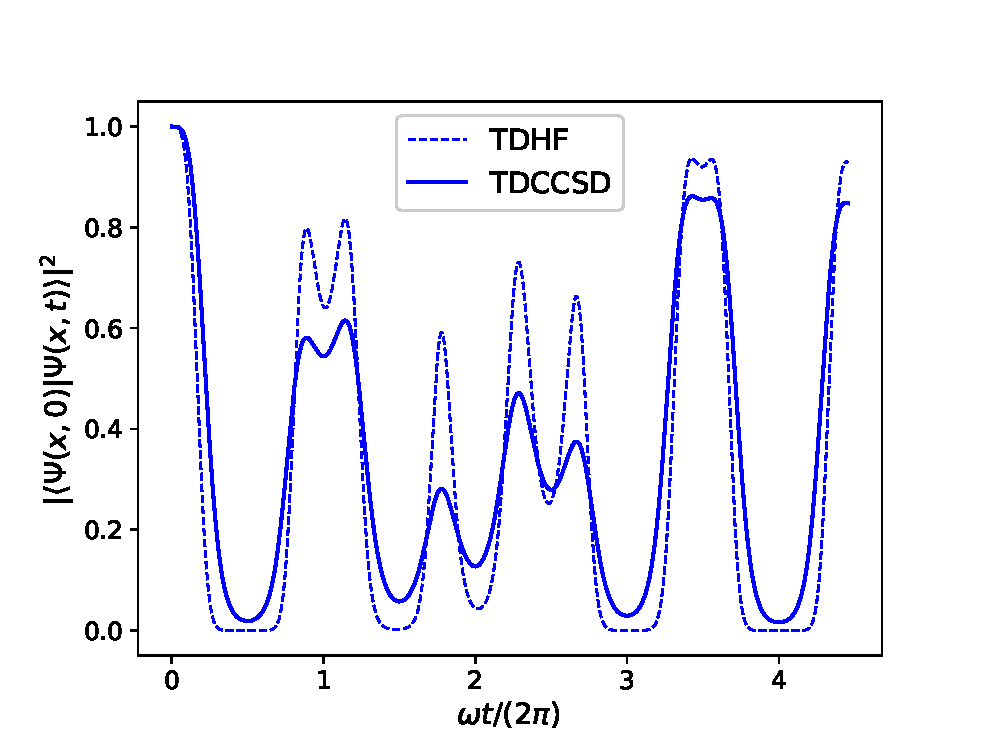
\includegraphics[width=0.5\textwidth]{./figures/zanghellini_fig2.eps}
        \caption{\label{fig:1DZanghellini} Probability of being in the ground state
        $|\langle\Psi(x,0\ket{\Psi(x,t)}|^2$ for one-dimensional quantum dot with frequency
        $\omega = 8\Omega$ and two electrons. This plot is an exact match with figure 2 in Zanghellini
        et al.\cite{Zanghellini04}
        }
        \end{figure}

    \subsection{Two-dimensional quantum dot calculations}
        Results from different interesting time-dependent observable quantities for distinct confining potentials and time-dependent fields (maybe too ambitious on different fields).

\section{Concluding remarks}
\begin{appendices}
\section{Derivation of TDHF equations} \label{TDHF_Derivation}
By introducing functional derivatives and their action on the matrix elements (see Hochstuhl et al \cite{Hochstuhl2014}),
\begin{align}
    \frac{\delta}{\delta \phi^*_k}\bra{\phi_i}\hat{h}\ket{\phi_i} &= \hat{h}\ket{\phi_k} \\
    \frac{\delta}{\delta \phi^*_k}\bra{\phi_i}\frac{\partial}{\partial t} \ket{\phi_i} 
    &= \frac{\partial}{\partial t}\ket{\phi_k} \\
    \frac{\delta}{\delta \phi^*_k}\bra{\phi_i \phi_j} \hat{u} \ket{\phi_i, \phi_j}_{\text{AS}}
    &= 2\bra{\cdot \phi_i} \hat{u} \ket{\phi_k \phi_i}_{\text{AS}},
\end{align}
one can find the equations of motions for the system by way of the time-dependent variational principle,
\begin{equation}
    \label{td_variational_principle}
    \bra{\delta \Phi} \hat{H} - i\hbar \frac{\partial}{\partial t} \ket{\Phi} = 0.
\end{equation}

(INSERT SHORT NOTE ON EMPTY SLOT NOTATION?)

We are faced with an optimisation problem under the constraint that the orbitals are orthonormal ($\braket{\phi_i(t)}{\phi_j(t)} = \delta_{ij})$, yielding the following Lagrange functional,
\begin{equation}
    \mathcal{L} = \bra{\Phi} \hat{H} - i\hbar \frac{\partial}{\partial t} \ket{\Phi} 
    - \lambda_{ij}(\braket{\phi_i(t)}{\phi_j(t)} - \delta_{ij}),
\end{equation}
with an optimal state $\ket{\phi_k}$ satisfying
\begin{equation}
    \label{HF_optimal_phi}
    \hat{h}\ket{\phi_k} + \bra{\cdot \phi_j} \hat{u} \ket{\phi_k \phi_j}_{\text{AS}} 
    - i\hbar\frac{\partial}{\partial t} \ket{\phi_k} - \lambda_{kj} \ket{\phi_j} = 0.
\end{equation}
Left-projecting this expression onto a state $\bra{\phi_l}$ and solving for the lagrange multiplier $\lambda$ gives
\begin{equation}
    \lambda_{kl} = \bra{\phi_l} \hat{h} \ket{\phi_k} 
    + \bra{\phi_l \phi_j} \hat{u} \ket{\phi_k \phi_j}_{\text{AS}}
    - i\hbar \bra{\phi_l} \frac{\partial}{\partial t} \ket{\phi_k}.
\end{equation}
Inserting this expression into \autoref{HF_optimal_phi} yields
\begin{equation}
    i\hbar \hat{P}\frac{\partial}{\partial t} \ket{\phi_k} = \hat{P} \hat{f} \ket{\phi_k},
\end{equation}
where we have defined a projection opertor $\hat{P} = \mathbb{1} - \ket{\phi_i}\bra{\phi_i}$ and the Fock operator $\hat{f} \equiv \hat{h} + \bra{\cdot \phi_j} \hat{u} \ket{\cdot \phi_j}_{\text{AS}}$.

For unitary time-dependent operator given by $\hat{Q}(t) = i\hbar (\partial / \partial t)$,
we have
\begin{equation}
    \label{TDHF}
    i \hbar \frac{\partial}{\partial t} \ket{\phi_k(t)} = \hat{f} \ket{\phi_k(t)},
\end{equation}
if we choose $\hat{Q}(t) = \hat{f}(t)$. \autoref{TDHF} is the time-dependent Hartree-Fock equations, which can be rewritten on matrix form by expanding the molecular slater wavefunctions in an atomic basis with time-dependent coefficients and left projecting with an arbitrary atomic basis function,
\begin{align}
    i \hbar \frac{\partial}{\partial t} C_{\alpha i} (t) \ket{\chi_\alpha} &= \hat{f}(t) C_{\alpha i} (t) \ket{\chi_\alpha} \\
    \to i \hbar \frac{\partial}{\partial t} C_{\alpha i} (t) \langle{\chi_{\beta}}|{\chi_{\alpha}}\rangle &= C_{\alpha i}(t) \bra{\chi_\beta} \hat{f}(t) \ket{\chi_\alpha} \\
    \to i \hbar \mathbf{S}\dot{\mathbf{C}}(t) &= \mathbf{F}(t) \mathbf{C}(t).
\end{align}
\section{The time dependent energy}
In general the time dependent energy is given by 
\begin{equation}
    E(t) = \braket{\Psi(t)|\hat{H}(t)|\Psi(t)}.
\end{equation}
If $\hat{H}$ does not depend explicitly on time, we find that the energy is conserved
\begin{align*}
     \frac{\partial}{\partial t}E(t) &= \braket{\frac{\partial \Psi(t)}{\partial t}|\hat{H}|\Psi(t)} + \braket{\Psi(t)|\hat{H}|\frac{\partial \Psi(t)}{\partial t}} \\
     &= \braket{\Psi(t)|\hat{H}|\frac{\partial \Psi(t)}{\partial t}}^* + \braket{\Psi(t)|\hat{H}|\frac{\partial \Psi(t)}{\partial t}} \\
     &= (-i\braket{\Psi(t)|\hat{H}^2|\Psi(t)})^* -i\braket{\Psi(t)|\hat{H}^2|\Psi(t)} \\
     &= 0
\end{align*}
where we used the time dependent Schrödinger equation 
\begin{equation}
    i \frac{\partial \Psi(t)}{\partial t}  = \hat{H} \Psi(t)
\end{equation}
to obtain the last equalities.
\section{Semi-analytical solutions for two electrons confined by a harmonic oscillator potential}
We review the (semi)-analytical solution(s) of two electrons confined by a harmonic oscillator potential as discussed by Taut \cite{Taut93,Taut94}, in two- and three spatial dimensions. We also consider the analogous one dimensional problem. 

Consider the Hamiltonian for two interacting particles in a harmonic oscillator potential, 
\begin{equation}
    \hat{H} = \sum_{i=1}^2 \left(\frac{1}{2} \mathbf{p}_i^2 + \frac{1}{2} \Omega^2 \mathbf{r}_i^2\right) + v_{\text{int}}(\mathbf{r}_1,\mathbf{r}_2). 
\end{equation}
In one spatial dimension the interaction between the electrons is modelled by a smoothed Coulomb potential \cite{SmoothedCoulomb} 
\begin{equation}
    v_{\text{int}}(x_1,x_2) = \frac{1}{\sqrt{(x_1-x_2)^2 + a^2}}
\end{equation}
where $a$ is a shielding parameter. In two- or three spatial dimensions the interaction is given by the usual Coulomb potential.

Following Taut \cite{Taut93} we introduce the difference vector and the center of mass as new variables,
\begin{align}
    \mathbf{r} &= \mathbf{r}_2-\mathbf{r}_1 \\
    \mathbf{R} &= \frac{1}{2} \left( \mathbf{r}_1+\mathbf{r}_2 \right). 
\end{align}
The key observation is that the Hamiltonian decouples in these variables
\begin{align}
    H &= - \nabla_\mathbf{r}^2 + \frac{1}{4} \Omega^2 \mathbf{r}^2 + v_{\text{int}}(\mathbf{r})  - \frac{1}{4}\nabla_\mathbf{R}^2 + \Omega^2 \mathbf{R}^2 \nonumber \\
    &= 2 \left( -\frac{1}{2} \nabla_\mathbf{r}^2 + \frac{1}{2} \Omega_\mathbf{r}^2 \mathbf{r}^2 + \frac{1}{2}v_{\text{int}}(\mathbf{r}) \right) \nonumber \\  &+ \frac{1}{2} \left( -\frac{1}{2}\nabla_\mathbf{R}^2 + \frac{1}{2}\Omega_\mathbf{R}^2 \mathbf{R}^2 \right) \nonumber \\
    &= 2 H_\mathbf{r} + \frac{1}{2}H_\mathbf{R} 
\end{align}
where we have defined 
\begin{align}
    \Omega_\mathbf{r} &\equiv \frac{1}{2}\Omega \\
    \Omega_\mathbf{R} &\equiv 2 \Omega \\
    H_\mathbf{r} &\equiv -\frac{1}{2} \nabla_\mathbf{r}^2   + \frac{1}{2} \Omega_\mathbf{r}^2 \mathbf{r}^2 + \frac{1}{2}v_{\text{int}}(\mathbf{r}) \\
    H_\mathbf{R} &\equiv -\frac{1}{2}\nabla_\mathbf{R}^2 + \frac{1}{2}\Omega_\mathbf{R}^2 \mathbf{R}^2
\end{align}
Since $H$ is independent of spin, the total wave function can be factorized as follows\cite{Taut93} 
\begin{equation}
    \psi(\mathbf{r},\mathbf{R},\mathbf{s}) = \varphi(\mathbf{r}) \xi(\mathbf{R}) \chi(s_1,s_2).
\end{equation}
Thus, the time-independent Schrödinger equation 
\begin{align}
    H\psi(\mathbf{r},\mathbf{R},\mathbf{s}) &= \left( 2 H_\mathbf{r} + \frac{1}{2}H_\mathbf{R} \right) \varphi(\mathbf{r}) \xi(\mathbf{R}) \chi(s_1,s_2) \\ 
    &= E\psi(\mathbf{r},\mathbf{R},\mathbf{s}) \\
    &= \left( E_\mathbf{r} + E_\mathbf{R} \right) \varphi(\mathbf{r}) \xi(\mathbf{R}) \chi(s_1,s_2)
\end{align}
separates into one equation for the relative motion
\begin{equation}
    \left[- \frac{1}{2}\nabla_\mathbf{r}^2 + \frac{1}{2} \omega_r^2 \mathbf{r}^2 + \frac{1}{2}v_{\text{int}}(\mathbf{r}) \right] \varphi(\mathbf{r}) = E^\prime_\mathbf{r} \varphi(\mathbf{r}) \label{RelativeMotionEquation}
\end{equation}
where $E^\prime_\mathbf{r} = \frac{1}{2}E_\mathbf{r}$, and one for the center of mass 
\begin{equation}
    \left[- \frac{1}{2}\nabla_\mathbf{R}^2 + \frac{1}{2}\Omega_R^2 \mathbf{R}^2 \right] = E^\prime_\mathbf{R} \xi(\mathbf{R}) \label{CenterOfMassEquation}
\end{equation}
where $E^\prime_\mathbf{R} = 2 E_\mathbf{R}$. The total energy is then given by 
\begin{equation}
    E = E_\mathbf{r} + E_\mathbf{R} = 2E^\prime_\mathbf{r} + \frac{1}{2}E^\prime_\mathbf{R}.
\end{equation}

We recognize equation (\ref{CenterOfMassEquation}) as the eigenvalue problem for a (d-dimensional) harmonic oscillator with frequency $\Omega_R$.Thus, 
\begin{equation}
    E_\mathbf{R}^\prime = \Omega_\mathbf{R} \left( n_d + \frac{d}{2} \right)
\end{equation}
for $d=1,2,3$.

In one dimension we can solve the eigenvalue problem for the relative motion (\ref{RelativeMotionEquation}) numerically, with the smoothed Coulomb potential, using for example a finite difference discretization.

In the next section we discuss how to solve the equation for the relative motion i two spatial dimensions.   

\section{Solving the two-dimensional Schrödinger equation for a central symmetric potential}
Consider the Schrödinger equation in two dimensions for a central symmetric potential where we use polar coordinates 
\begin{equation}
    \left[ - \frac{1}{2} \nabla^2_{r,\theta} + V(r) \right] \psi(r,\theta) = E\psi(r,\theta). \label{SEPolar}
\end{equation}
The Laplacian in polar coordinates is given by
\begin{equation}
    \nabla_{r,\theta}^2 = \frac{1}{r} \frac{\partial}{\partial r} \left( r \frac{\partial}{\partial r} \right) + \frac{1}{r^2} \frac{\partial^2}{\partial \theta^2}
\end{equation}

Inserting the expressions for the Laplacian into equation (\ref{SEPolar}) we have that
\begin{equation}
    \left[ - \frac{1}{2} \left(\frac{1}{r} \frac{\partial}{\partial r} \left( r \frac{\partial}{\partial r} \right) + \frac{1}{r^2} \frac{\partial^2}{\partial \theta^2} \right) + V(r) \right] \psi(r,\theta) = E\psi(r,\theta).
\end{equation}

We look for solutions that are seprable on the form
\begin{equation}
    \psi(r,\theta) = R(r) \varphi(\theta)
\end{equation}
such that
\begin{equation*}
     - \frac{1}{2} \left(\frac{\varphi}{r} \frac{\partial}{\partial r} \left( r \frac{\partial R}{\partial r} \right) + \frac{R}{r^2} \frac{\partial^2 \varphi}{\partial \theta^2} \right) + V(r)R\varphi   = ER\varphi.
\end{equation*}

Multiplying with $-2r^2$ and dividing with $R\varphi$ we obtain
\begin{equation*}
      \left[\frac{r}{R}\frac{\partial}{\partial r} \left( r \frac{\partial R}{\partial r} \right) -2r^2 (V(r)-E) \right] + \frac{1}{\varphi} \frac{\partial^2 \varphi}{\partial \theta^2}     = 0,
\end{equation*}
which implies that 
\begin{equation}
    \frac{r}{R}\frac{\partial}{\partial r} \left( r \frac{\partial R}{\partial r} \right) -2r^2 (V(r)-E) = m^2 \end{equation}
    and
    \begin{equation}
    \frac{1}{\varphi} \frac{\partial^2 \varphi}{\partial \theta^2} = -m^2.
\end{equation}

\subsection{The angular equation}
The second (angular) equation is satisfied by 
\begin{equation}
    \varphi = Ne^{im\theta}
\end{equation}
with $N$ a normalization constant. Requiring 
\begin{equation}
    \varphi(\theta + 2\pi) = \varphi(\theta)
\end{equation}
implies that $m=0,\pm 1, \pm 2,\cdots$. The normalization condition 
\begin{equation}
\int_0^{2\pi} |\varphi|^2 d\theta = 2\pi|N|^2 = 1    
\end{equation} gives $N = 1/\sqrt{2\pi}$.

\subsection{The radial equation}
Next, we consider the radial equation
\begin{equation}
    r\frac{\partial}{\partial r} \left( r \frac{\partial R}{\partial r} \right) -2r^2 (V(r)-E)R = Rm^2 \label{2d-RadialEquation}
    \end{equation}
This equation simplifies if we change variables
\begin{equation}
    R(r) = \frac{u(r)}{r^{1/2}}
\end{equation}
and note that 
\begin{equation}
    r\frac{\partial}{\partial r} \left( r \frac{\partial R}{\partial r} \right) = r^{-1/2} \left[ r^2 \frac{d^2 u}{dr} + \frac{1}{4}u(r) \right].
\end{equation}
Insertion in equation (\ref{2d-RadialEquation}) yields
\begin{equation}
    \left[ -\frac{1}{2} \frac{d^2}{dr^2} + \frac{1}{2r^2} \left( m^2 - \frac{1}{4} \right) + V(r) \right] u(r) = Eu(r) \label{2d-radial-new}.
\end{equation}

For two interacting particles confined by a harmonic oscillator potential the potential is given by 
\begin{equation}
    V(r) = \frac{1}{2}\Omega_r^2 + \frac{1}{2r},
\end{equation}
for which equation (\ref{2d-radial-new}) can be solved analytically for particular oscillator frequencies\cite{Taut94}. 

One can also solve the equation numerically for arbitrary oscillator frequencies. The main challenge in a numerical approach is how to deal with the singularities at $r=0$.

\section{Semi-analytical solution of a laser-driven two electron system}
Following Schwengelbeck \cite{SCHWENGELBECK_1999} we consider the problem of two interacting electrons, confined by a harmonic oscillator potential, subject to a time-dependent sinusoidal laser-field. The Hamiltonian of the system is given by 
\begin{equation}
    \hat{H} = \sum_{i=1}^2 \left(\frac{1}{2} \mathbf{p}_i^2 + \frac{1}{2} \Omega^2 r_i^2 + \mathbf{r}_i \cdot \hat{\mathbf{e}} E_0 \sin(\omega t)  \right) + v_{\text{int}}(\mathbf{r}_1,\mathbf{r}_2). 
\end{equation}
where $\omega$ and $E_0$ are the frequency and amplitude of the field and $\hat{\mathbf{e}}$ denotes a unit polarization vector.

As in the previous section, introducting the relative distance and center of mass as new variables, the Hamiltonian decouples
\begin{align}
    H &= 2 \underbrace{\left( -\frac{1}{2} \nabla_\mathbf{r}^2 + \frac{1}{2} \Omega_\mathbf{r}^2 \mathbf{r}^2 + \frac{1}{2}v_{\text{int}}(\mathbf{r}) \right)}_{\equiv H_\mathbf{r}} \nonumber \\  &+ \frac{1}{2} \underbrace{\left( -\frac{1}{2}\nabla_\mathbf{R}^2 + \frac{1}{2}\Omega_\mathbf{R}^2 \mathbf{R}^2 + 4\mathbf{R} \cdot \hat{\mathbf{e}} E_0 \sin(\omega t) \right)}_{\equiv H_\mathbf{R}}
\end{align}
and the time-dependent Schrödringer equation admits solutions of the factorized form\cite{SCHWENGELBECK_1999}
\begin{equation}
    \Psi(\mathbf{r},\mathbf{R},\mathbf{s},t) = \psi(\mathbf{R},t) \varphi(\mathbf{r},t) \chi(s_1,s_2).
\end{equation}
We use the ground state of the unperturbed system as initial condition
\begin{equation}
    \Psi(\mathbf{r},\mathbf{R},\mathbf{s},0) = \psi_0(\mathbf{R},0) \varphi_0(\mathbf{r},0) \chi(s_1,s_2),
\end{equation}
where $\varphi_0(\mathbf{r})$ and $\psi_0(\mathbf{R})$ are the ground state solutions of equations (\ref{RelativeMotionEquation}) and (\ref{CenterOfMassEquation}) respectively.

In particular, we get one equation for the relative motion 
\begin{equation}
    i \frac{\partial}{\partial t} \varphi(\mathbf{r},t) = 2H_\mathbf{r} \varphi(\mathbf{r},t)
\end{equation}
and one for the center of mass
\begin{equation}
    i \frac{\partial}{\partial t} \psi(\mathbf{R},t) = \frac{1}{2}H_\mathbf{R} \psi(\mathbf{R},t) \label{time-dependent CM eq}.
\end{equation}
Since $H_\mathbf{r}$ contains no explicit time-dependent terms, the equation for the relative motion is simply given by 
\begin{equation}
    \varphi(\mathbf{r},t) = \varphi_0(\mathbf{r},0) \exp(-i E^\prime_{0,\mathbf{r}} t)
\end{equation}
where $\{(\phi_0(\mathbf{r},0),E^\prime_{0,\mathbf{r}}\}$ is given by the lowest lying solution of equation (\ref{RelativeMotionEquation}).

\subsection{Solving the center of mass equation in time}
Eq. (\ref{time-dependent CM eq}) associated with the center of mass motion of the two electrons, can be solved analytically by means of a path integral\cite{SCHWENGELBECK_1999} or we can use a numerical approach. 

\subsubsection{One spatial dimension}
Consider first the one dimensional problem, $(\mathbf{r},\mathbf{R}) = (x,X)$ with polarization vector $\hat{\mathbf{e}}$ along the positive x-direction 
\begin{align}
    i \frac{\partial \psi(X,t)}{\partial t} &= \frac{1}{2} H_X(t) \psi(X,t) \label{OneDimTimeDepEq}
\end{align}
where 
\begin{equation}
    H_X(t) =  -\frac{1}{2}\frac{d^2}{dX^2} + \frac{1}{2}\Omega_X^2 X^2 + 4X \sin(\omega t) 
\end{equation}
and $\Omega_X \equiv 2\Omega$. We use the ground state of the unperturbed harmonic oscillator as initial state for center of mass wavefunction 
\begin{equation}
    \psi(X,0) = \left( \frac{\Omega_X}{\pi} \right)^{1/4} \exp\left(-\frac{\Omega_X X^2}{2}\right).
\end{equation}
Equation (\ref{OneDimTimeDepEq}) is solved by using the standard Runge-Kutta fourth order (RK4) scheme.

Thus, we have that the total wavefunction is given by 
\begin{align}
 \Psi(x,X,t) &= \varphi(x,t) \psi(X,t) \nonumber \\
 &= \varphi_0(x,0)e^{-tiE_{0,x}^\prime} \psi(X,t).
\end{align}
where $E_{0,x}^\prime$ is the lowest eigenvalue of for the relative coordinate equation (\ref{RelativeMotionEquation}).

We will use this solution to benchmark the more general many-body solvers. In particular, we can compute the expectation value 
of the time-dependent Hamiltonian
\begin{align}
 \braket{\Psi|\hat{H}|\Psi} &= \braket{\Psi|H_x|\Psi} + \braket{\Psi|H_X(t)|\Psi} \nonumber \\
 &= E_{0,x}^\prime + \braket{\Psi|H_X(t)|\Psi}.
\end{align}

\subsubsection{Two spatial dimensions}
The two dimensional problem is almost a carbon copy of the one dimensional problem. We have that $\mathbf{R} = (X,Y)$ and we choose the polarization vector $\hat{\mathbf{e}}$ along the positive x-direction
\begin{align*}
    i \frac{\partial \psi(\mathbf{R},t)}{\partial t} &= \left( -\frac{1}{4}\nabla_\mathbf{R}^2 + \Omega^2 \mathbf{R}^2 + 2\mathbf{R} \cdot \hat{\mathbf{e}} \sin(\omega t) \right) \psi(\mathbf{R},t) \\
    &= \frac{1}{2}\underbrace{\left( -\frac{1}{2}\nabla_\mathbf{R}^2 + \frac{1}{2}\Omega_R^2 \mathbf{R}^2 + 2X \sin(\omega t) \right)}_{\equiv H_\mathbf{R}} \psi(\mathbf{R},t)
\end{align*}
where we again have that $\Omega_R = 2\Omega$.

Since we have chosen the polarization axis along the positive x-direction (or y-direction) the Hamiltonian separates
\begin{align*}
    H_\mathbf{R} &= \frac{1}{2}\left( -\frac{1}{2}\frac{\partial^2}{\partial X^2} + \frac{1}{2}\Omega_R^2 \mathbf{X}^2 + 2X \sin(\omega t) -\frac{1}{2}\frac{\partial^2}{\partial Y^2} + \frac{1}{2}\Omega_R^2 \mathbf{Y}^2 \right) \\
    &= \frac{1}{2}(H_X(t) + H_Y).
\end{align*}
Note that $H_Y$ does not contain any explicit time-dependent terms.

Then, the time-dependent Schrödinger equation for the center of mass motion admits solutions of the factorized form
\begin{equation}
    \psi(\mathbf{R},t) = \psi(X,Y,t) = \psi_X(X,t) \psi_Y(Y,t).
\end{equation}
We use the ground state of the unperturbed two-dimensional harmonic oscillator as intial condition
\begin{align}
    \psi(X,Y,0) = &\left( \frac{\Omega_R}{\pi} \right)^{1/4} \exp\left(-\frac{\Omega_R X^2}{2}\right) \nonumber \\ 
    \times &\left( \frac{\Omega_R}{\pi} \right)^{1/4} \exp\left(-\frac{\Omega_R Y^2}{2}\right)
\end{align}

Insertion of this ansatz into the time-dependent Schrödinger equation yields two independent equations 
\begin{align}
    i \frac{\partial \psi_X}{\partial t} &= \frac{1}{2} H_X(t) \psi_X \\
    i \frac{\partial \psi_Y}{\partial t} &= \frac{1}{2} H_Y \psi_Y. 
\end{align}
The first equation is now formally equivalent to the one-dimensional problem. 

The second equation has the solution of a unperturbed one-dimensional harmonic oscillator 
\begin{equation}
    \psi_Y(Y,t) = \psi(y) e^{-i \epsilon_{0,Y} t}
\end{equation}
where \begin{equation}
    \epsilon_{0,y} = \frac{1}{2}\eta_Y
\end{equation} 
 and 
\begin{equation}
    \eta_Y = \frac{1}{2}\Omega_R
\end{equation}
is the ground state energy of a harmonic oscillator with oscillator frequency $\Omega_R$.

Finally, we have that the total wavefunction is given by 
\begin{align}
 \Psi(\mathbf{r},\mathbf{R},t) &= \varphi(\mathbf{r},t) \psi(\mathbf{R},t) \nonumber \\
 &= \varphi(\mathbf{r},0)e^{-i\epsilon t} \psi_X(X,t) \psi_Y(Y,t).
\end{align}
where $\epsilon$ is the lowest eigenvalue of for the relative coordinate equation (\ref{RelativeMotionEquation}) in two spatial dimensions.

In particular, we find that the expectation value of the time-dependent Hamiltonian is given by 
\begin{align}
    \braket{\Psi|\hat{H}|\Psi} &= \braket{\Psi|\hat{H}_\mathbf{r}|\Psi} + \braket{\Psi|H_\mathbf{R}|\Psi} \nonumber \\ 
    &= \epsilon + \braket{\Psi|H_Y|\Psi} + \braket{\Psi|H_X(t)|\Psi} \nonumber \\
    &= \epsilon + \epsilon_{0,y} + \braket{\Psi|H_X(t)|\Psi}.
\end{align}

\section{The harmonic potential theorem}
The harmonic potential theorem: See Dobson\cite{HarmonicPotentialTheorem} and section 6.3.2 in the book by Ullrich\cite{TD_DFT_Ullrich_Book}.


\end{appendices}
\newpage
\bibliographystyle{ieeetr}
\bibliography{refs}
\end{document}
